\documentclass[12pt]{article}
\usepackage[
backend=biber,
style=abnt,
sorting=nyt
]{biblatex}
\usepackage{csquotes}
\addbibresource{bibliografia.bib}
\AtBeginBibliography{\raggedright \footnotesize}
\setlength{\bibitemsep}{\baselineskip}

\usepackage{amsmath} %Para usar símbolos matemáticos

\usepackage[brazil]{babel} %Para usar a linguagem português
\addto\captionsbrazil{
    \renewcommand{\contentsname}{\texorpdfstring{\normalsize SUMÁRIO}{SUMÁRIO}}
    \renewcommand{\listtablename}{\texorpdfstring{\normalsize ÍNDICE DE TABELAS}{ÍNDICE DE TABELAS}}
    \renewcommand{\listfigurename}{\texorpdfstring{\normalsize ÍNDICE DE FIGURAS}{ÍNDICE DE FIGURAS}}
}

\usepackage{subcaption}
\usepackage{float}
\usepackage{graphicx} %Para inserir imagens
\usepackage{geometry} %Para alterar propriedades da página
\geometry{
a4paper,
left=30mm,
top=30mm,
right=20mm,
bottom=20mm
}

\usepackage[hidelinks]{hyperref}

\usepackage{tocloft}
\renewcommand{\cfttoctitlefont}{\hfill}
\renewcommand{\cftaftertoctitle}{\hfill}
\renewcommand{\cftsecfont}{\normalsize\normalfont\bfseries}
\renewcommand{\cftsubsecindent}{0pt}
\renewcommand{\cftsubsecfont}{\normalsize\normalfont}
\renewcommand{\cftsubsubsecindent}{0pt}
\renewcommand{\cftsubsubsecfont}{\normalsize\normalfont\bfseries}
\renewcommand{\cftsecleader}{\cftdotfill{\cftdotsep}}
\renewcommand{\cftlottitlefont}{\hfill} %Centralizar o título da lista de tabelas
\renewcommand{\cftafterlottitle}{\hfill}
\renewcommand{\cfttabpresnum}{Tabela\ } %Adicionar Tabela antes do nome de cada item
\renewcommand{\cfttabaftersnum}{:\ }
\setlength{\cfttabnumwidth}{4.75em}
\renewcommand{\cftdotsep}{1}
\renewcommand{\cftloftitlefont}{\hfill}
\renewcommand{\cftafterloftitle}{\hfill}
\renewcommand{\cftfigpresnum}{Figura\ }
\renewcommand{\cftfigaftersnum}{:\ }
\setlength{\cftfignumwidth}{4.75em}

\usepackage{titlesec}
\titleformat{\section}{\normalsize\bfseries\MakeUppercase}{\thesection}{0.5em}{}
\titleformat{\subsection}{\normalsize\MakeUppercase}{\thesubsection}{0.5em}{}
\titleformat{\subsubsection}{\normalsize\bfseries}{\thesubsubsection}{0.5em}{}

\usepackage{fancyhdr}
\pagestyle{fancy}
\fancyhf{} % Limpa os cabeçalhos e rodapés
\fancyhead[R]{\footnotesize\thepage} % Coloca o número da página no canto superior direito
\fancyfoot[C]{} % Remove qualquer número de página no rodapé
\renewcommand{\headrulewidth}{0pt} % Remove a linha horizontal do cabeçalho
\renewcommand{\footrulewidth}{0pt} % Remove a linha horizontal do rodapé

\usepackage{multicol}
\usepackage{pgfplots}
\pgfplotsset{compat=1.18}
\usepackage[american]{circuitikz}
\usetikzlibrary{external}\tikzexternalize
\usetikzlibrary{positioning}

\usepackage{setspace} %Para alterar o espaçamento das linhas
\setstretch{1.5}

\begin{document}
    \begin{titlepage}
    \begin{center}
        \large
        Universidade Federal do Espírito Santo - UFES\\
        Departamento de Computação e Eletrônica - DCEL\\
        Engenharia de Computação
        
        \vfill
        \textbf{
        Relatório da experiência 01\\
        Resistores\\~\\
        }
        
        Disciplina: Circuitos Elétricos I\\
        Prof. Flávio Duarte Couto Oliveira\\
        
        \vfill
        \begin{flushright}
            Pedro Henrique Alves do Nascimento
        \end{flushright}
        
        \vfill
        Espírito Santo\\
        Dezembro 2024
    \end{center}
    \newpage
\end{titlepage}
    
    % \listoftables
    % \thispagestyle{empty}
    % \newpage

    \listoffigures
    \thispagestyle{empty}
    \newpage

    \tableofcontents
    \thispagestyle{empty}
    \newpage

    \section*{Pedro Henrique Alves do Nascimento}
    \section{INTRODUÇÃO TEÓRICA}
    \subsection{RESISTORES EM SÉRIE}
    É definido que quando somente dois elementos de circuito estão ligados ao mesmo nó, eles estão em série, é fácil ver, aplicando a Lei de Kirchhoff das Correntes em cada nó, que elementos em série conduzem a mesma corrente \parencite[][, p. 61]{nilsson}, como mostrado na Figura \ref{fig:r-serie}.

    \begin{figure}[H]
        \centering
        \caption{Resistores ligados em série.}
        \begin{tikzpicture}
            \ctikzset{nodes width=0.06}
            \draw (0,0) node[below] {$h$} to [R, l=$R_7$, *-*, v<=$ $] (3,0) node[below] {$g$} to
            [R, l=$R_6$, -*, v<=$ $] (6,0) node[below] {$f$} to
            [R, l=$R_5$, -*, v<=$ $] (9,0) node[below] {$e$} to
            [R, l_=$R_4$, -*, v<=$ $] (9,3) node[above] {$d$} to
            [R, l_=$R_3$, -*, v^<=$ $] (6,3) node[above] {$c$} to
            [R, l_=$R_2$, -*, v^<=$ $] (3,3) node[above] {$b$} to
            [R, l_=$R_1$, v^<=$ $, -*] (0,3) node[above] {$a$} to
            [voltage source, v_=$v_s$, f<=$i_s$, sources/scale=1.5] (0,0);
        \end{tikzpicture}
        \label{fig:r-serie}
    \end{figure}
    
    Além disso, com a Lei de Kirchhoff das Tensões, é possível ver que $n$ resistores em série podem ser substituídos por um único resistor equivalente de resistência $R_{eq}$, conforme mostrados nas Equações \ref{eq:parte-1-serie} e \ref{eq:parte-2-serie} e na Figura \ref{fig:r-serie-equivalente}.
    \begin{gather}
        -v_s+i_sR_1+i_sR_2+i_sR_3+i_sR_4+i_sR_5+i_sR_6+i_sR_7=0 \label{eq:parte-1-serie}\\
        v_s=i_s\left(R_1+R_2+R_3+R_4+R_5+R_6+R_7\right)\implies v_s=i_s\cdot R_{eq} \label{eq:parte-2-serie}
    \end{gather}

    \begin{figure}[H]
        \centering
        \caption{Resistor em série equivalente.}
        \begin{tikzpicture}
            \ctikzset{nodes width=0.06}
            \draw (0,0) to [short, *-] (3,0) to
            [R, l_=$R_{eq}$, v^<=$ $] (3,3) to
            [short, -*] (0,3) node[above] {$a$} to
            [voltage source, v_=$v_s$, f<=$i_s$, sources/scale=1.5] (0,0) node[below] {$h$};
        \end{tikzpicture}
        \label{fig:r-serie-equivalente}
    \end{figure}

    \subsection{RESISTORES EM PARALELO}
    Dois elementos de circuito estão ligados em paralelo quando seus terminais estão ligados a um único par de nós. Elementos ligados em paralelo têm a mesma tensão em seus terminais \parencite[][, p. 62]{nilsson}. A Figura \ref{fig:r-paralelo} mostra ligações desse tipo.
    \begin{figure}[H]
        \centering
        \caption{Resistores em paralelo.}
        \begin{tikzpicture}
            \ctikzset{nodes width=0.06}
            \draw (1,0) to [short, -*] (3,0) node[below] {$b$} to
            [short, -*] (5,0) to
            [R, l_=$R_1$, -*] (5,3) to
            [short, -*] (3,3) node[above] {$a$} to
            [short] (1,3) to
            [voltage source, v_=$v_s$, sources/scale=1.5, f<=$i_s$] (1,0);
            \draw (5,0) to [short, -*] (7,0) to
            [R, l_=$R_2$, -*] (7,3) to
            [short] (5,3);
            \draw (7,0) to [short] (9,0) to
            [R, l_=$R_3$] (9,3) to
            [short] (7,3);
        \end{tikzpicture}
        \label{fig:r-paralelo}
    \end{figure}

    A Lei de Kirchhoff das correntes nos informa que $i_s=i_1+i_2+i_3$, sendo $i_n$ a corrente que passa pelo resistor $R_n$, essa informação é utilizada na Equação \ref{eq:req-paralelo}.
    Uma característica dos resistores em paralelo é que eles podem ser reduzidos a um resistor equivalente de resistência $R_{eq}$ por meio da Equação \ref{eq:req-paralelo}.
    \begin{equation}
        \label{eq:req-paralelo}
        \frac{i_s}{v_s}=\frac{1}{R_{eq}}=\frac{1}{R_1}+\frac{1}{R_2}+\frac{1}{R_3}
    \end{equation}

    Desenvolvendo essa expressão, facilmente chega-se à Equação \ref{eq:produto-soma}, que é utilizada quando há somente dois resistores ligados em paralelo.
    \begin{equation}
        \label{eq:produto-soma}
        R_1\parallel R_2 = R_{eq}=\frac{R_1\cdot R_2}{R_1+R_2}
    \end{equation}

    \section{AULA PRÁTICA}
    \subsection{PARTE 1}
    Foram utilizados quatro resistores com valor nominal de 180 $\Omega$, 470 $\Omega$, 820 $\Omega$ e 1,2 k$\Omega$, ligados conforme a Figura \ref{fig:circuito-parte1} em uma protoboard, e um multímetro na escala de resistência para medição da resistência equivalente entre os terminais $a$ e $e$.
    \begin{figure}[H]
        \centering
        \caption{Circuito da 1ª parte da aula prática.}
        \begin{tikzpicture}
            \ctikzset{nodes width=0.06}
            \draw (0,0) node [above] {$a$} to [R,l={180 $\Omega$}, *-*] (2,0) node [above] {$b$} to
            [R, l={470 $\Omega$}, -*] (4,0) node [above] {$c$} to
            [R, l={1,2 k$\Omega$}, -*] (6,0) node [above] {$d$} to
            [R, l={820 $\Omega$}, -*] (8,0) node [above] {$e$};
        \end{tikzpicture}
        \label{fig:circuito-parte1}
    \end{figure}

    \begin{figure}[H]
        \centering
        \caption{Circuito 1 montado em laboratório.}
        \begin{minipage}{0.5\textwidth}
            \centering
            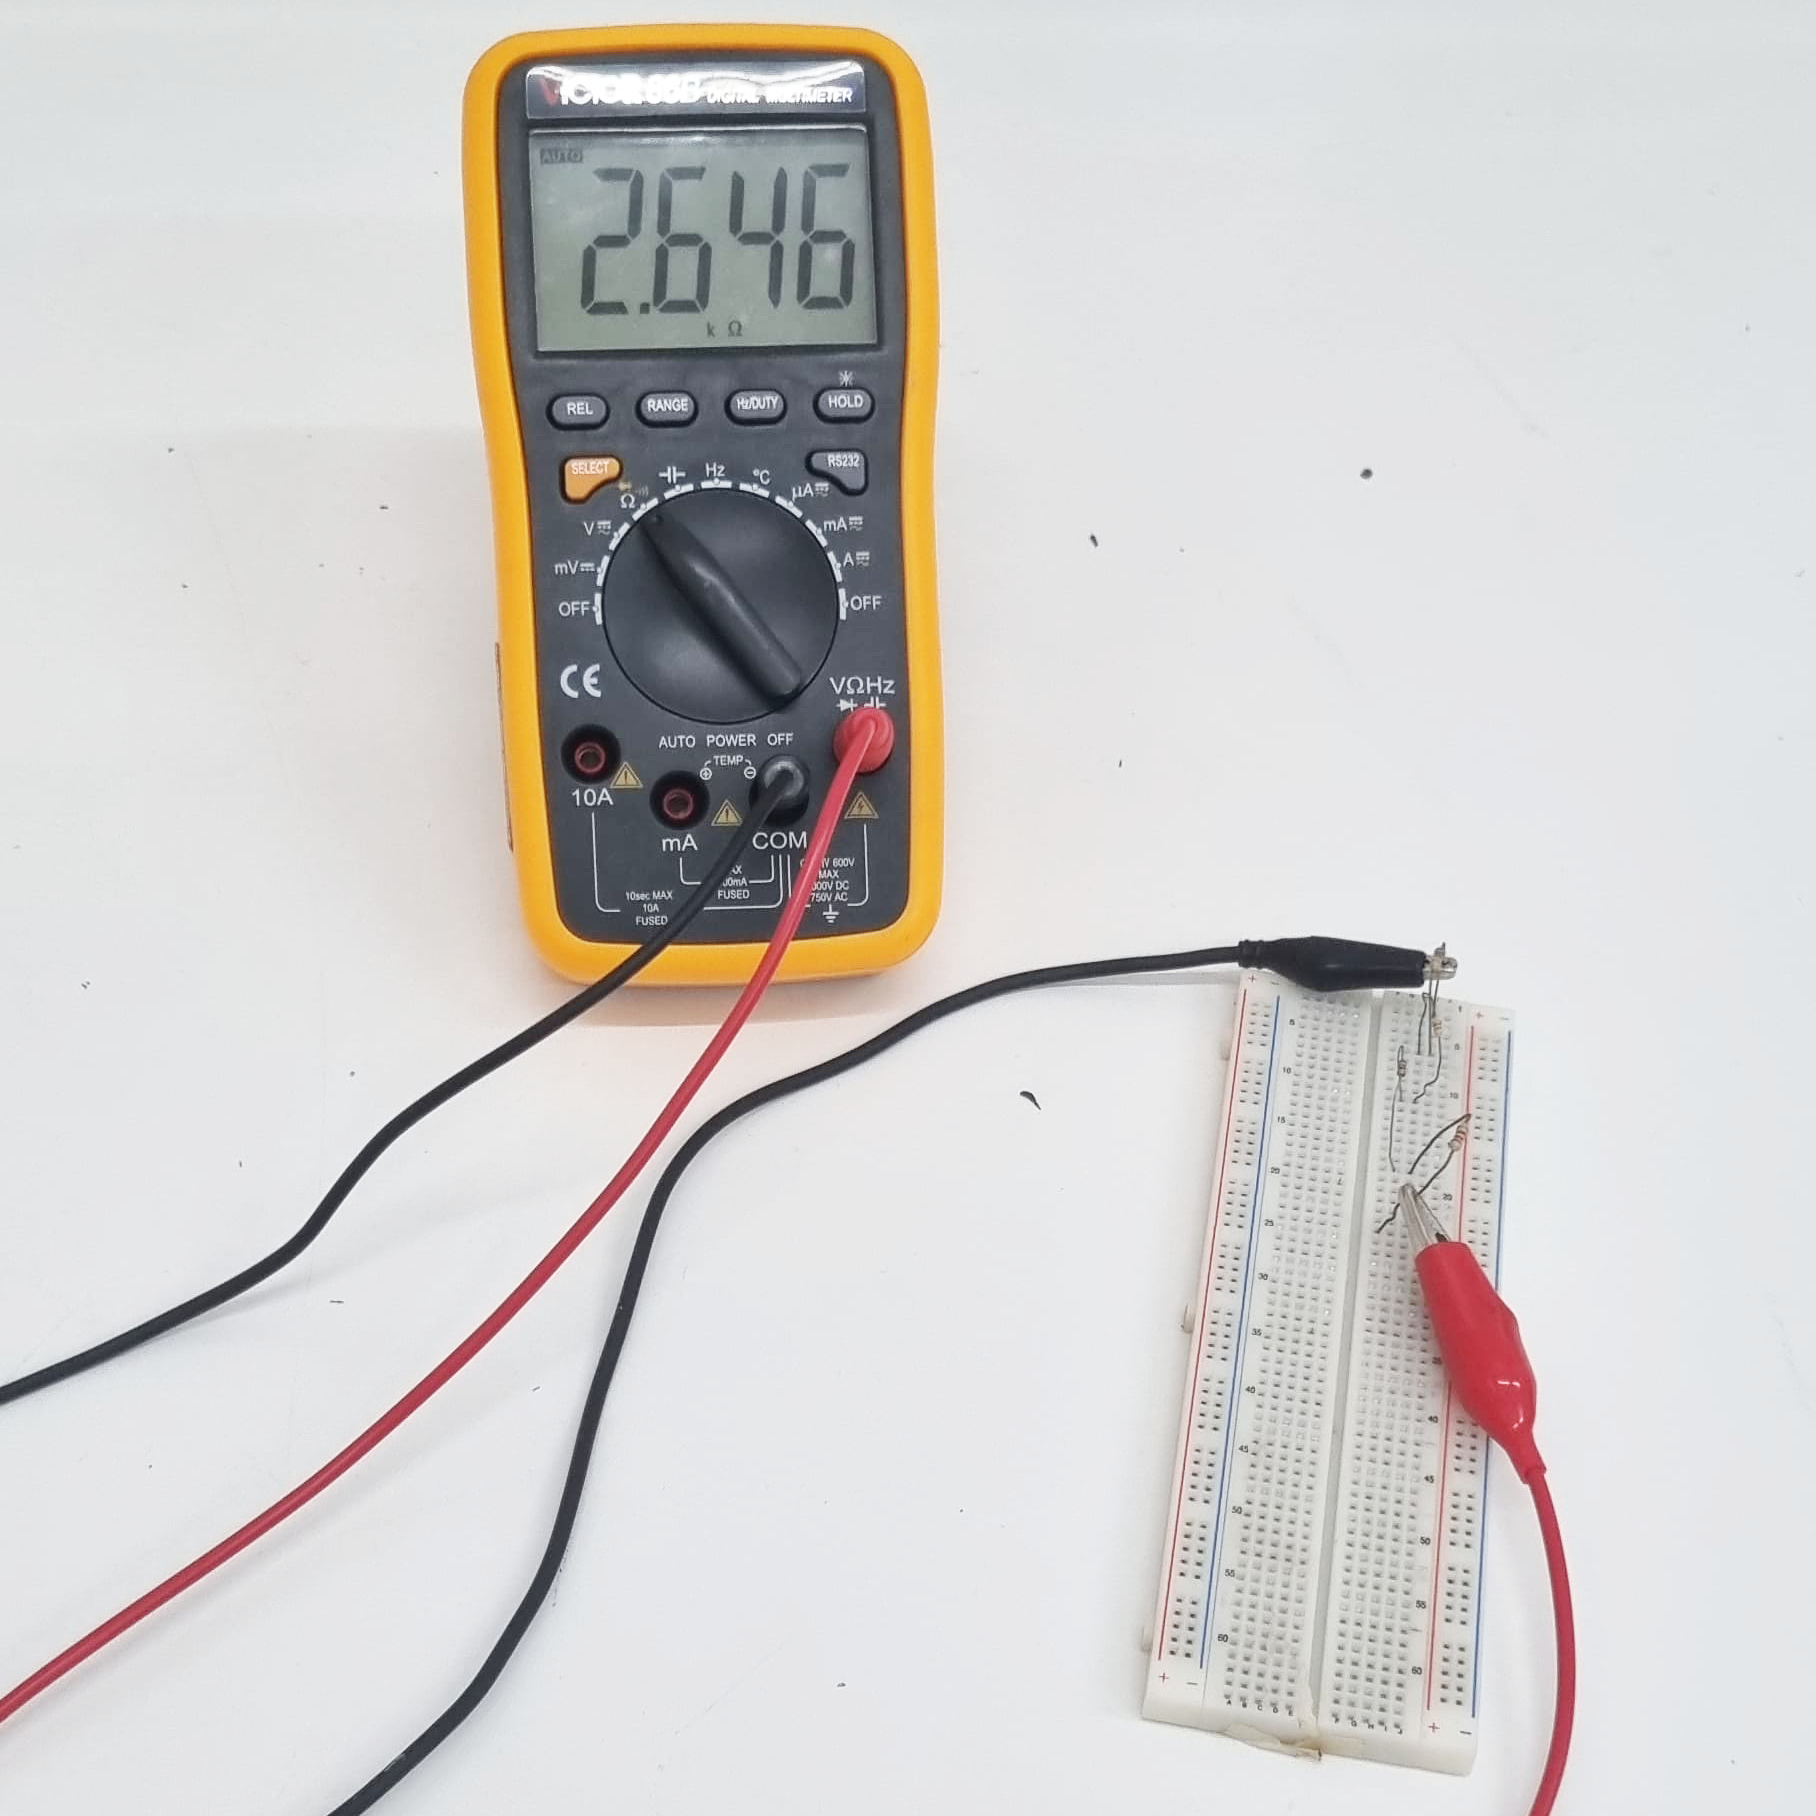
\includegraphics[width=\textwidth]{external-figures/parte1.png}\\
            \raggedright\footnotesize{Fonte: Elaborado pelo autor.}
            \label{fig:pratica1}
        \end{minipage}
    \end{figure}

    Mediu-se, então, a resistência entre os terminais $a$ e $e$, encontrando $R_{ae(medida)}=2,646\text{ k}\Omega$. Calculou-se, então, a resistência equivalente entre os terminais $a$ e $e$ utilizando a Equação \ref{fig:r-serie-equivalente} conforme segue:
    \begin{align*}
        R_{ae(calculada)}&=180 + 470 + 1200 + 820\\
        R_{ae(calculada)}&=2,670\text{ k}\Omega
    \end{align*}

    O erro de medição encontrado, portanto, foi de $-$0,90\%.

    \subsection{PARTE 2}
    De maneira similar a parte 1, foi montado o circuito conforme Figura \ref{fig:circuito-parte2} e mediu-se e calculou-se suas resistências equivalentes entre $a$ e $b$. A resistência medida foi de $R_{ab(medida)}=236,6\ \Omega$.
    \begin{figure}[H]
        \centering
        \caption{Circuito da 2ª parte da aula prática.}
        \begin{tikzpicture}
            \ctikzset{nodes width=0.06}
            \draw (0,0) to [short, -*] (2,0) node [below] {$b$} to
            [R, l_={1,2 k$\Omega$}, -*] (2,3) node [above] {$a$} to
            [short] (0,3) to
            [R, l={470 $\Omega$}] (0,0);
            \draw (2,0) to [short] (4,0) to
            [R, l_={820 $\Omega$}] (4,3) to
            [short] (2,3);
        \end{tikzpicture}
        \label{fig:circuito-parte2}
    \end{figure}

    \begin{figure}[H]
        \centering
        \caption{Circuito 2 montado em laboratório.}
        \begin{minipage}{0.25\textwidth}
            \centering
            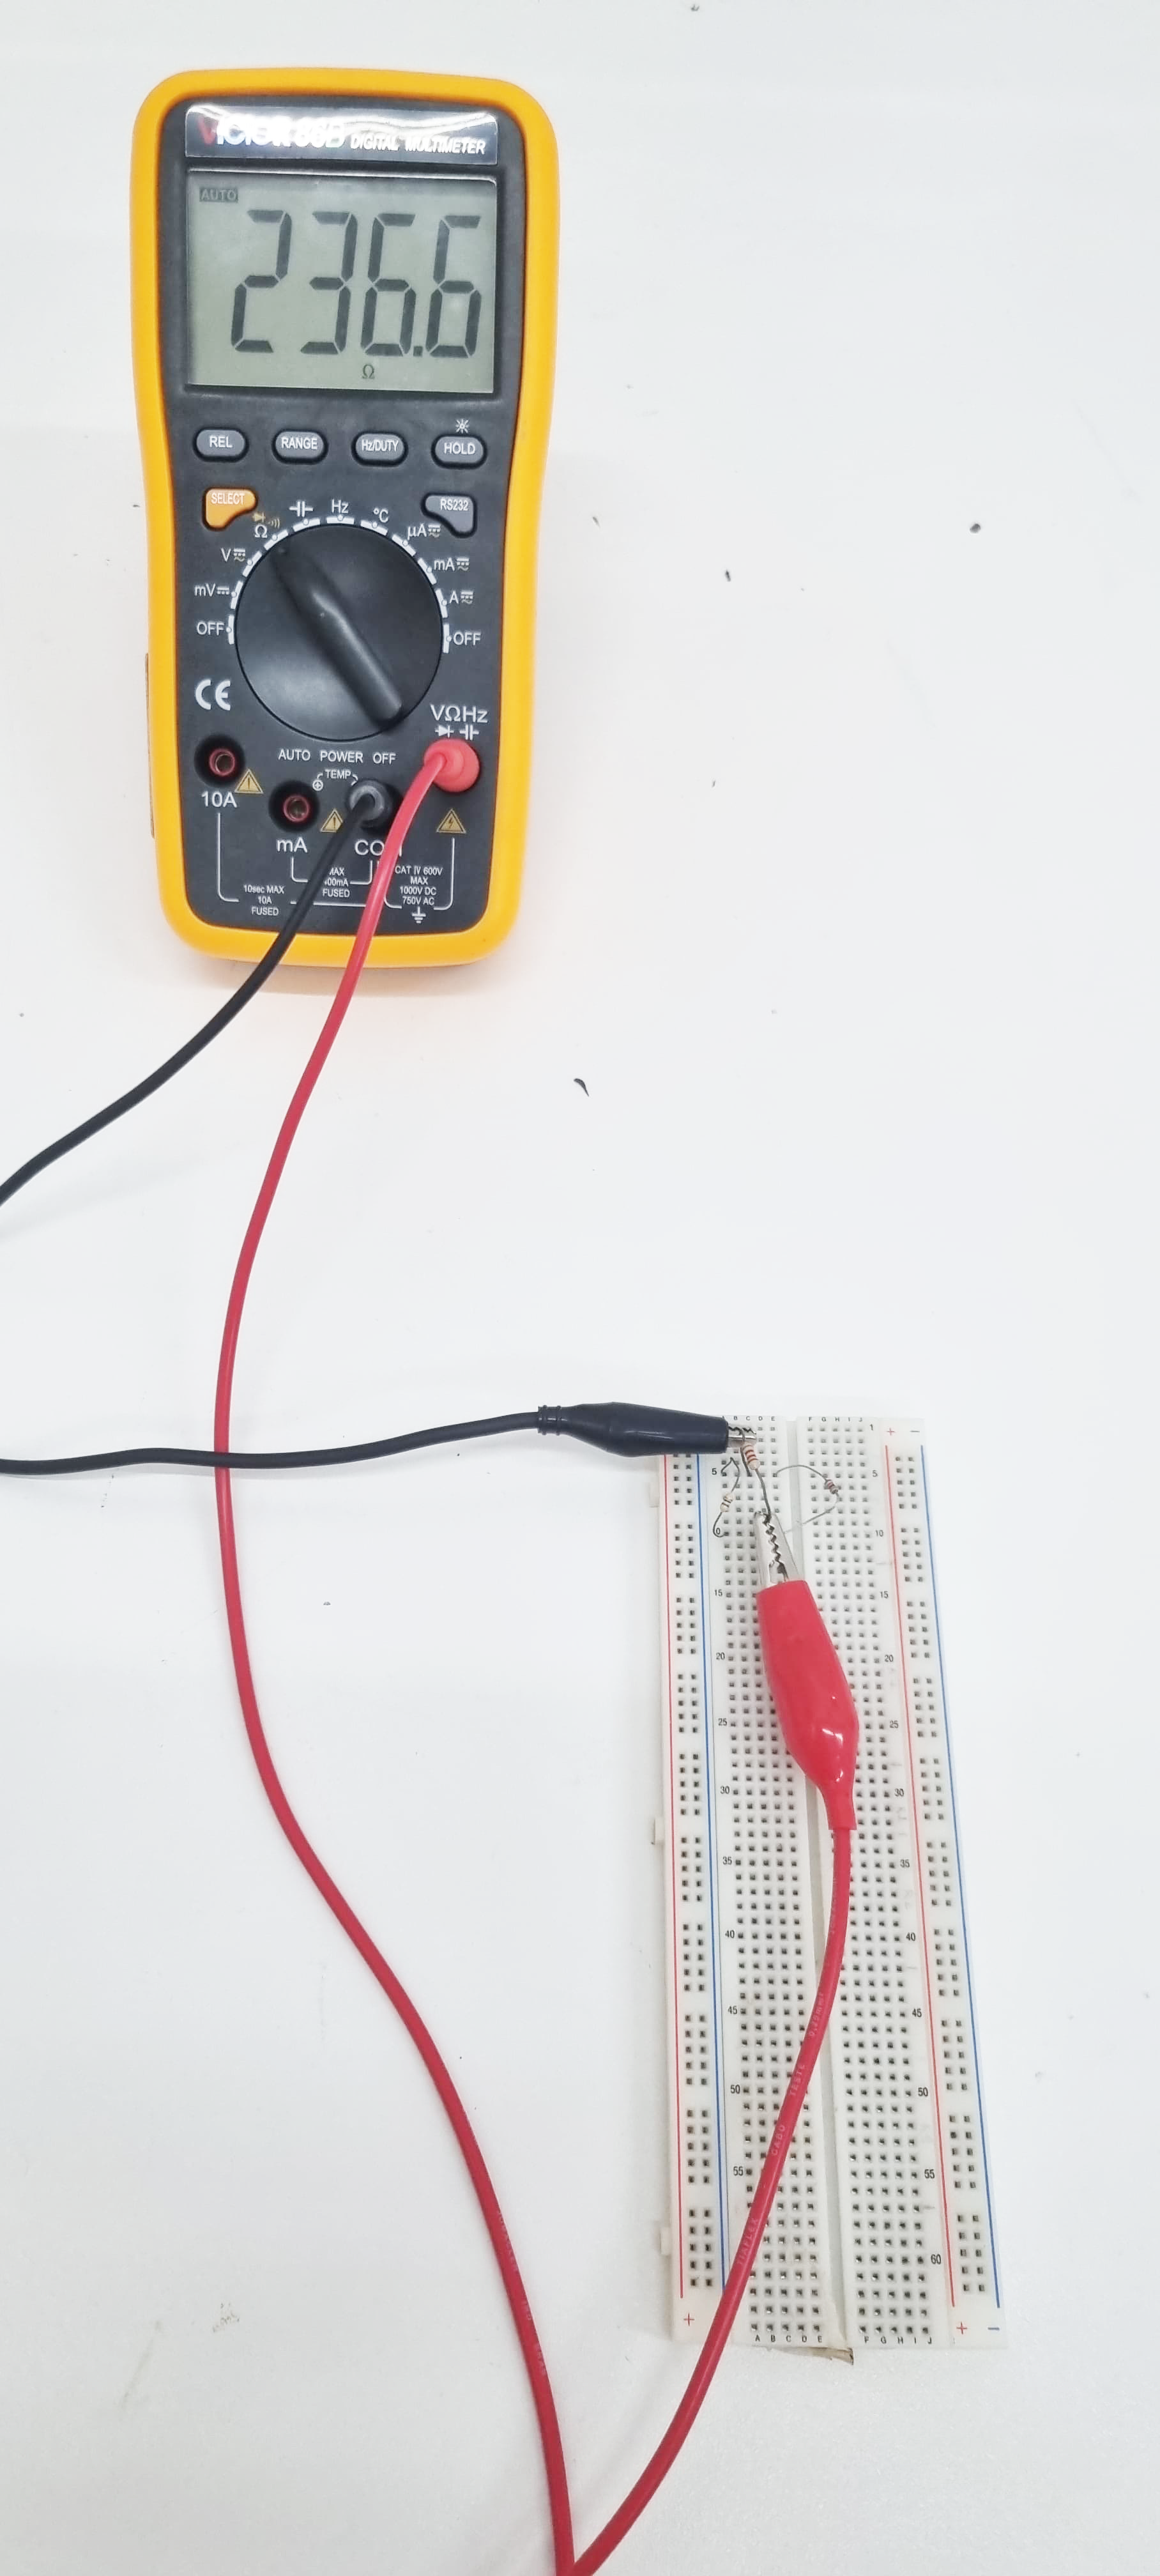
\includegraphics[width=\textwidth]{external-figures/parte2.png}\\
            \raggedright\footnotesize{Fonte: Elaborado pelo autor.}
            \label{fig:pratica2}
        \end{minipage}
    \end{figure}

    Calculou-se $R_{ab(calculada)}$ como segue:
    \begin{align*}
        R_{470\ \Omega}\parallel R_{1,2\text{ k}\Omega} &= \frac{470\cdot 1200}{470 + 1200} \approx 337,72\ \Omega \\
        R_{ab(calculada)}&=\frac{R_{470\ \Omega}\parallel R_{1,2\text{ k}\Omega}\cdot 820}{R_{470\ \Omega}\parallel R_{1,2\text{ k}\Omega} + 820}\\
        &=\frac{337,72\cdot 820}{337,72 + 820}\\
        R_{ab(calculada)}&=239,21\ \Omega
    \end{align*}

    O erro de medição foi, portanto, $-$1,09\%.

    \subsection{PARTE 3}
    Foi montado o circuito conforme Figura \ref{fig:circuito-parte3}, o valor medido foi $R_{ad(medida)}=1,999\text{ k}\Omega$.
    \begin{figure}[H]
        \centering
        \caption{Circuito da 3ª parte da aula prática.}
        \begin{tikzpicture}
            \ctikzset{nodes width=0.06}
            \draw (0,0) node [above] {$a$} to
            [R, l={1,2 k$\Omega$}, *-*] (3,0) node [above left] {$b$} to
            [short] (3,1) to
            [R, l={390 $\Omega$}] (5,1) to
            [R, l={470 $\Omega$}] (7,1) to
            [short, -*] (7,0) node [above right] {$c$} to
            [R, l=390 $\Omega$, -*] (10,0) node [above] {$d$};
            \draw (3,0) to [short] (3,-1) to
            [R, l={120 $\Omega$}] (5,-1) to
            [R, l={680 $\Omega$}] (7,-1) to
            (7,0);
        \end{tikzpicture}
        \label{fig:circuito-parte3}
    \end{figure}

    \begin{figure}[H]
        \centering
        \caption{Circuito 3 montado em laboratório.}
        \begin{minipage}{0.3\textwidth}
            \centering
            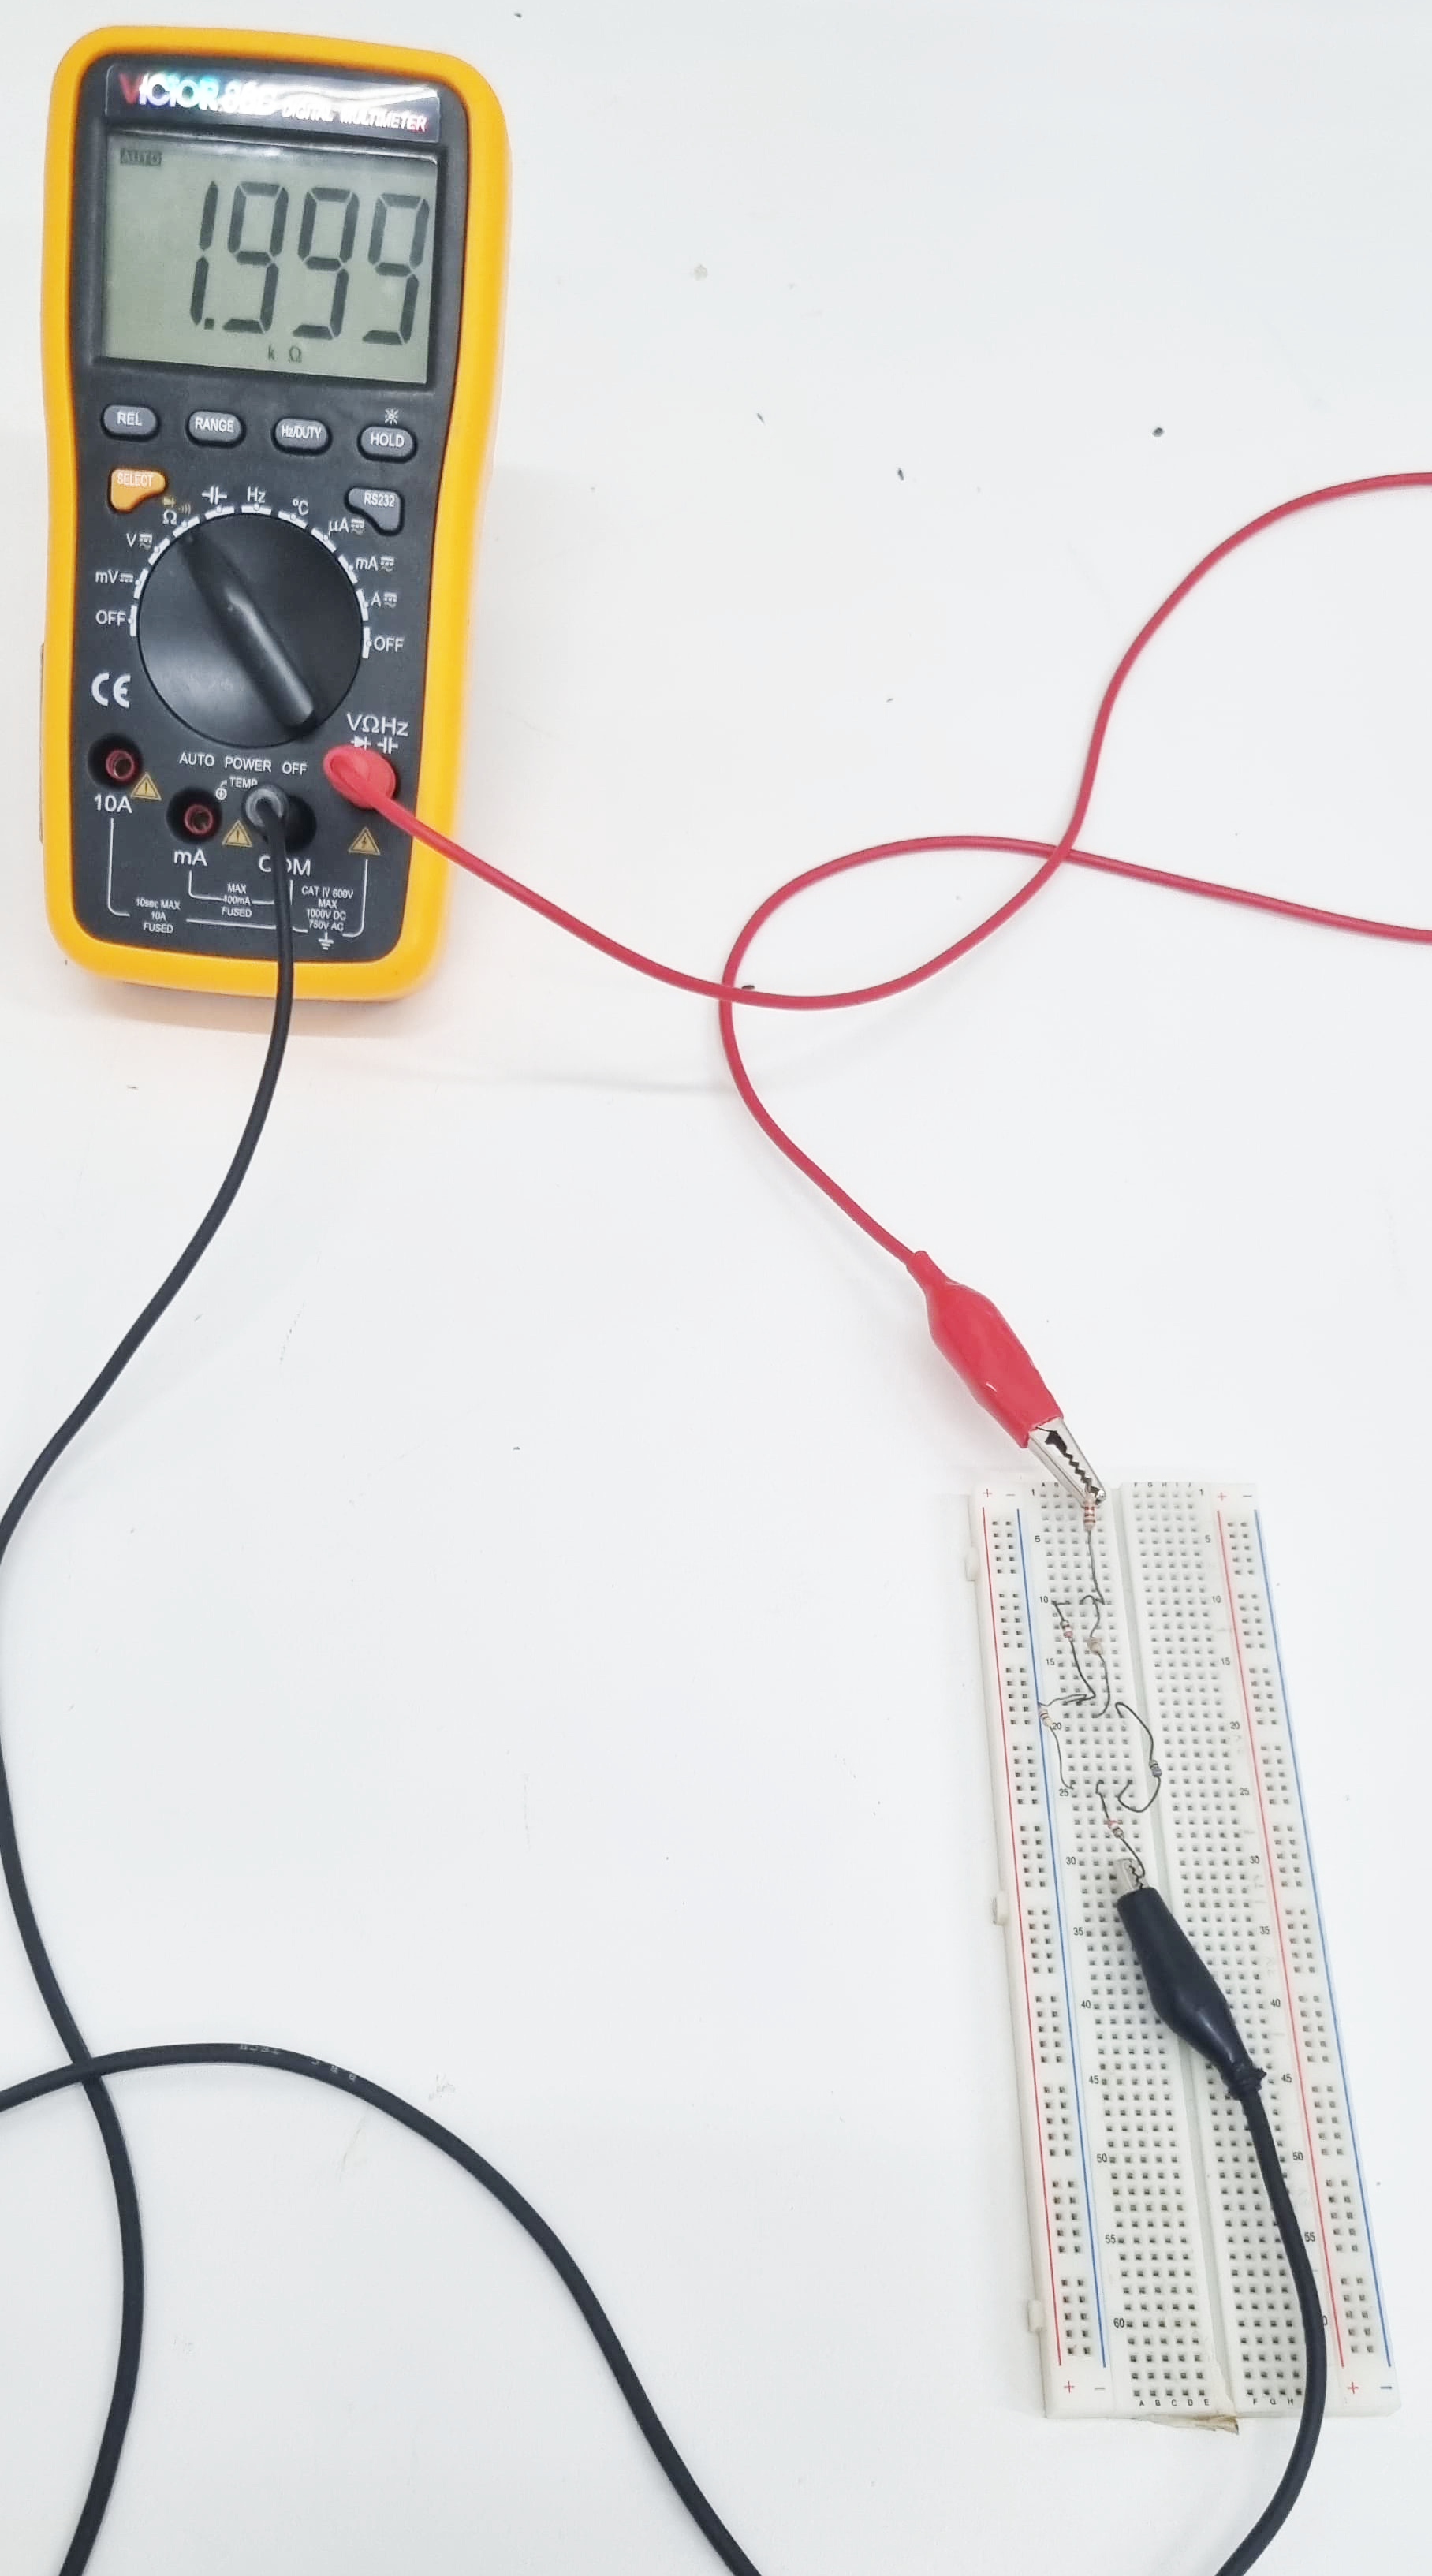
\includegraphics[width=\textwidth]{external-figures/parte3.png}\\
            \raggedright\footnotesize{Fonte: Elaborado pelo autor.}
            \label{fig:pratica3}
        \end{minipage}
    \end{figure}

    Calculou-se $R_{ad(calculada)}$ como segue:
    \begin{align*}
        R_{eq1}=390 + 470 &= 860\ \Omega\\
        R_{eq2}=120 + 680 &= 800\ \Omega\\
        R_{eq1}\parallel R_{eq2} = \frac{860\cdot 800}{860 + 800} &\approx 414,46\ \Omega\\
        R_{ab}=1200 + 414,46 + 390 &= 2004,46\ \Omega
    \end{align*}

    O erro de medição foi, portanto, $-$0,27\%.

    \section{CONCLUSÃO}
    Ao longo das medições realizadas nas três etapas da aula prática, foram observadas discrepâncias entre os valores de resistência medidos experimentalmente e os calculados teoricamente. Essas diferenças, embora relativamente pequenas (variando de $-$0,27\% a $-$1,09\%), podem ser atribuídas a diversos fatores. Entre os principais fatores que podem contribuir para tais discrepâncias estão:
    \begin{itemize}
        \item Imprecisões nos valores nominais dos resistores: Embora os resistores possuam valores especificados, a tolerância dos componentes pode gerar variações em relação ao valor nominal esperado;
        \item Instrumentação de medição: O multímetro utilizado possui uma margem de erro que pode influenciar os valores medidos.
    \end{itemize}  

    Ainda que os erros tenham sido baixos, a análise comparativa entre valores calculados e medidos ressalta a importância de considerar as limitações práticas durante a implementação de circuitos elétricos.

    \newpage
    \setstretch{1}
    \section*{\hfill REFERÊNCIAS BIBLIOGRÁFICAS\hfill}
    \addcontentsline{toc}{section}{REFERÊNCIAS BIBLIOGRÁFICAS}
    \printbibliography[heading=none]
\end{document}
